\section{Результаты исследования}

В рамках данной выпускной квалификационной работы было проведено комплексное исследование применимости нейроэволюционных алгоритмов для задачи моделирования поведения когнитивных агентов. Главный вектор исследования был направлен на концептуальный и эмпирический сравнительный анализ эволюционного подхода с классическими методами глубокого обучения с подкреплением.

Для максимально объективной оценки потенциала исследуемых алгоритмов была разработана методология поэтапного усложнения экспериментальных условий. Тестирование когнитивных моделей проводилось в трех симуляционных средах, каждая из которых предъявляла к агентам уникальные требования и обладала различной физикой взаимодействия:

\begin{enumerate}

  \item \textbf{CartPole} — базовая задача поддержания динамического равновесия, выступившая в роли фундаментального полигона для первичной проверки алгоритмов в дискретном пространстве действий.

  \item \textbf{LunarLander} — комплексная задача пространственного маневрирования, позволившая оценить способности агентов к микроконтролю, а также протестировать их устойчивость в условиях добавления внешних возмущений (имитация ветровых потоков и турбулентности).

  \item \textbf{Ant} — высокоуровневая задача непрерывного управления многокомпонентной биомеханической системой, продемонстрировавшая пределы применимости алгоритмов в многомерных пространствах.

\end{enumerate}

Оценка эффективности обученных агентов производилась не только по классическому критерию максимизации получаемой награды, но и с учетом таких критически важных для реальных систем параметров, как архитектурная сложность нейронной сети, скорость схождения и устойчивость к шумовым воздействиям.

Полученные в ходе симуляций экспериментальные данные позволили сформулировать ряд существенных выводов, описывающих сильные и слабые стороны каждого из подходов. Ниже представлены детализированные результаты исследования, систематизированные по каждой из рассмотренных сред моделирования.

\subsection{Результаты в среде CartPole}

Первым этапом экспериментального исследования стала классическая задача управления — балансировка перевернутого маятника (CartPole). Данная среда выступала в качестве фундаментального полигона для верификации работоспособности алгоритмов и оценки базовых характеристик когнитивных агентов. В рамках эксперимента проводилось сопоставление классического алгоритма глубокого Q-обучения (DQN) и нейроэволюционного метода (NEAT).

На этапе проектирования архитектур моделей были применены два принципиально разных подхода. Агент на базе DQN использовал фиксированную полносвязную нейронную сеть с одним скрытым слоем, содержащую 114 параметров. В противовес этому, алгоритм NEAT функционировал в парадигме постепенного усложнения (complexifying), начиная эволюционный процесс с простейшей топологии без скрытых слоев и динамически формируя структуру сети в ответ на требования среды.

Сравнительный анализ метрик (согласно определениям \ref{def:learning_efficiency}-\ref{def:robustness}) позволил сделать следующие ключевые выводы:


\subsubsection{Эффективность использования выборки и скорость схождения}

Оба алгоритма успешно справились с задачей, однако нейроэволюционный подход продемонстрировал существенно более высокую скорость адаптации. Алгоритму NEAT потребовалось всего 4 поколения (или 10 548 шагов взаимодействия со средой), чтобы найти оптимальную стратегию. В то же время алгоритму DQN для стабилизации весов и схождения потребовалось 471 эпизод, что эквивалентно 25 923 взаимодействиям. Таким образом, эволюционный алгоритм оказался более чем в 2,4 раза эффективнее с точки зрения затрат вычислительных тактов симуляции.


\subsubsection{Качество решения и архитектурная сложность}

В идеальных условиях обе модели достигли абсолютного максимума качества (средняя награда 500.00 из 500) со 100\% стабильностью (стандартное отклонение равно 0). Однако способы достижения этого результата кардинально различаются. В то время как DQN использует плотную полносвязную структуру (плотность связей 100\%), NEAT синтезировал высокоэффективную разреженную сеть, состоящую всего из 9 параметров (плотность связей 75\%). Это доказывает способность нейроэволюции находить экстремально компактные и легковесные решения, что критически важно для развертывания моделей на устройствах с ограниченными вычислительными ресурсами.


\subsubsection{Устойчивость к внешним возмущениям}

Наиболее значимое различие между алгоритмами было зафиксировано при стресс-тестировании агентов в условиях зашумленных данных. Для генерации шума в этом и последующий проектах используется Гауссовский шум. В данной среде берется стандартное отклонение равное 0.1. При добавлении шума в наблюдения среды, эффективность полносвязной модели DQN резко снизилась на 29,14\% (средняя награда упала до 354.30). Агент оказался склонен к переобучению под «идеализированную» картину мира. Напротив, агент NEAT продемонстрировал абсолютную робастность: в условиях аналогичного зашумления модель не потеряла ни одного балла, сохранив среднюю награду на уровне 500.00. Столь высокая устойчивость напрямую вытекает из компактности эволюционной архитектуры: из-за отсутствия «лишних» связей и параметров, сеть физически лишена способности пропускать через себя шумовые сигналы, фильтруя их на уровне самой топологии.


\subsubsection{Практические выводы}

Эксперимент в среде CartPole эмпирически доказал, что для решения базовых задач когнитивного управления нейроэволюционный алгоритм NEAT превосходит классический DQN по скорости схождения, компактности получаемой модели и, что наиболее важно, по уровню устойчивости к неопределенностям среды.

\subsection{Результаты в среде LunarLander}

Эксперименты в среде LunarLander стали ключевым этапом практического исследования, позволившим оценить работу когнитивных агентов в условиях сложного пространства состояний и необходимости тонкого микроконтроля. В отличие от базовой задачи CartPole, здесь перед агентами стояла цель не просто удержания баланса, а поиска оптимальной траектории посадки в условиях меняющейся гравитации и внешних возмущений.


\subsubsection{Сравнительный анализ архитектурной сложности и обучения}

В ходе исследования был зафиксирован значительный контраст в подходах к формированию управляющей политики:

\begin{figure}[h!] % [h!] - попытка разместить картинку "здесь" (here)
  \centering
  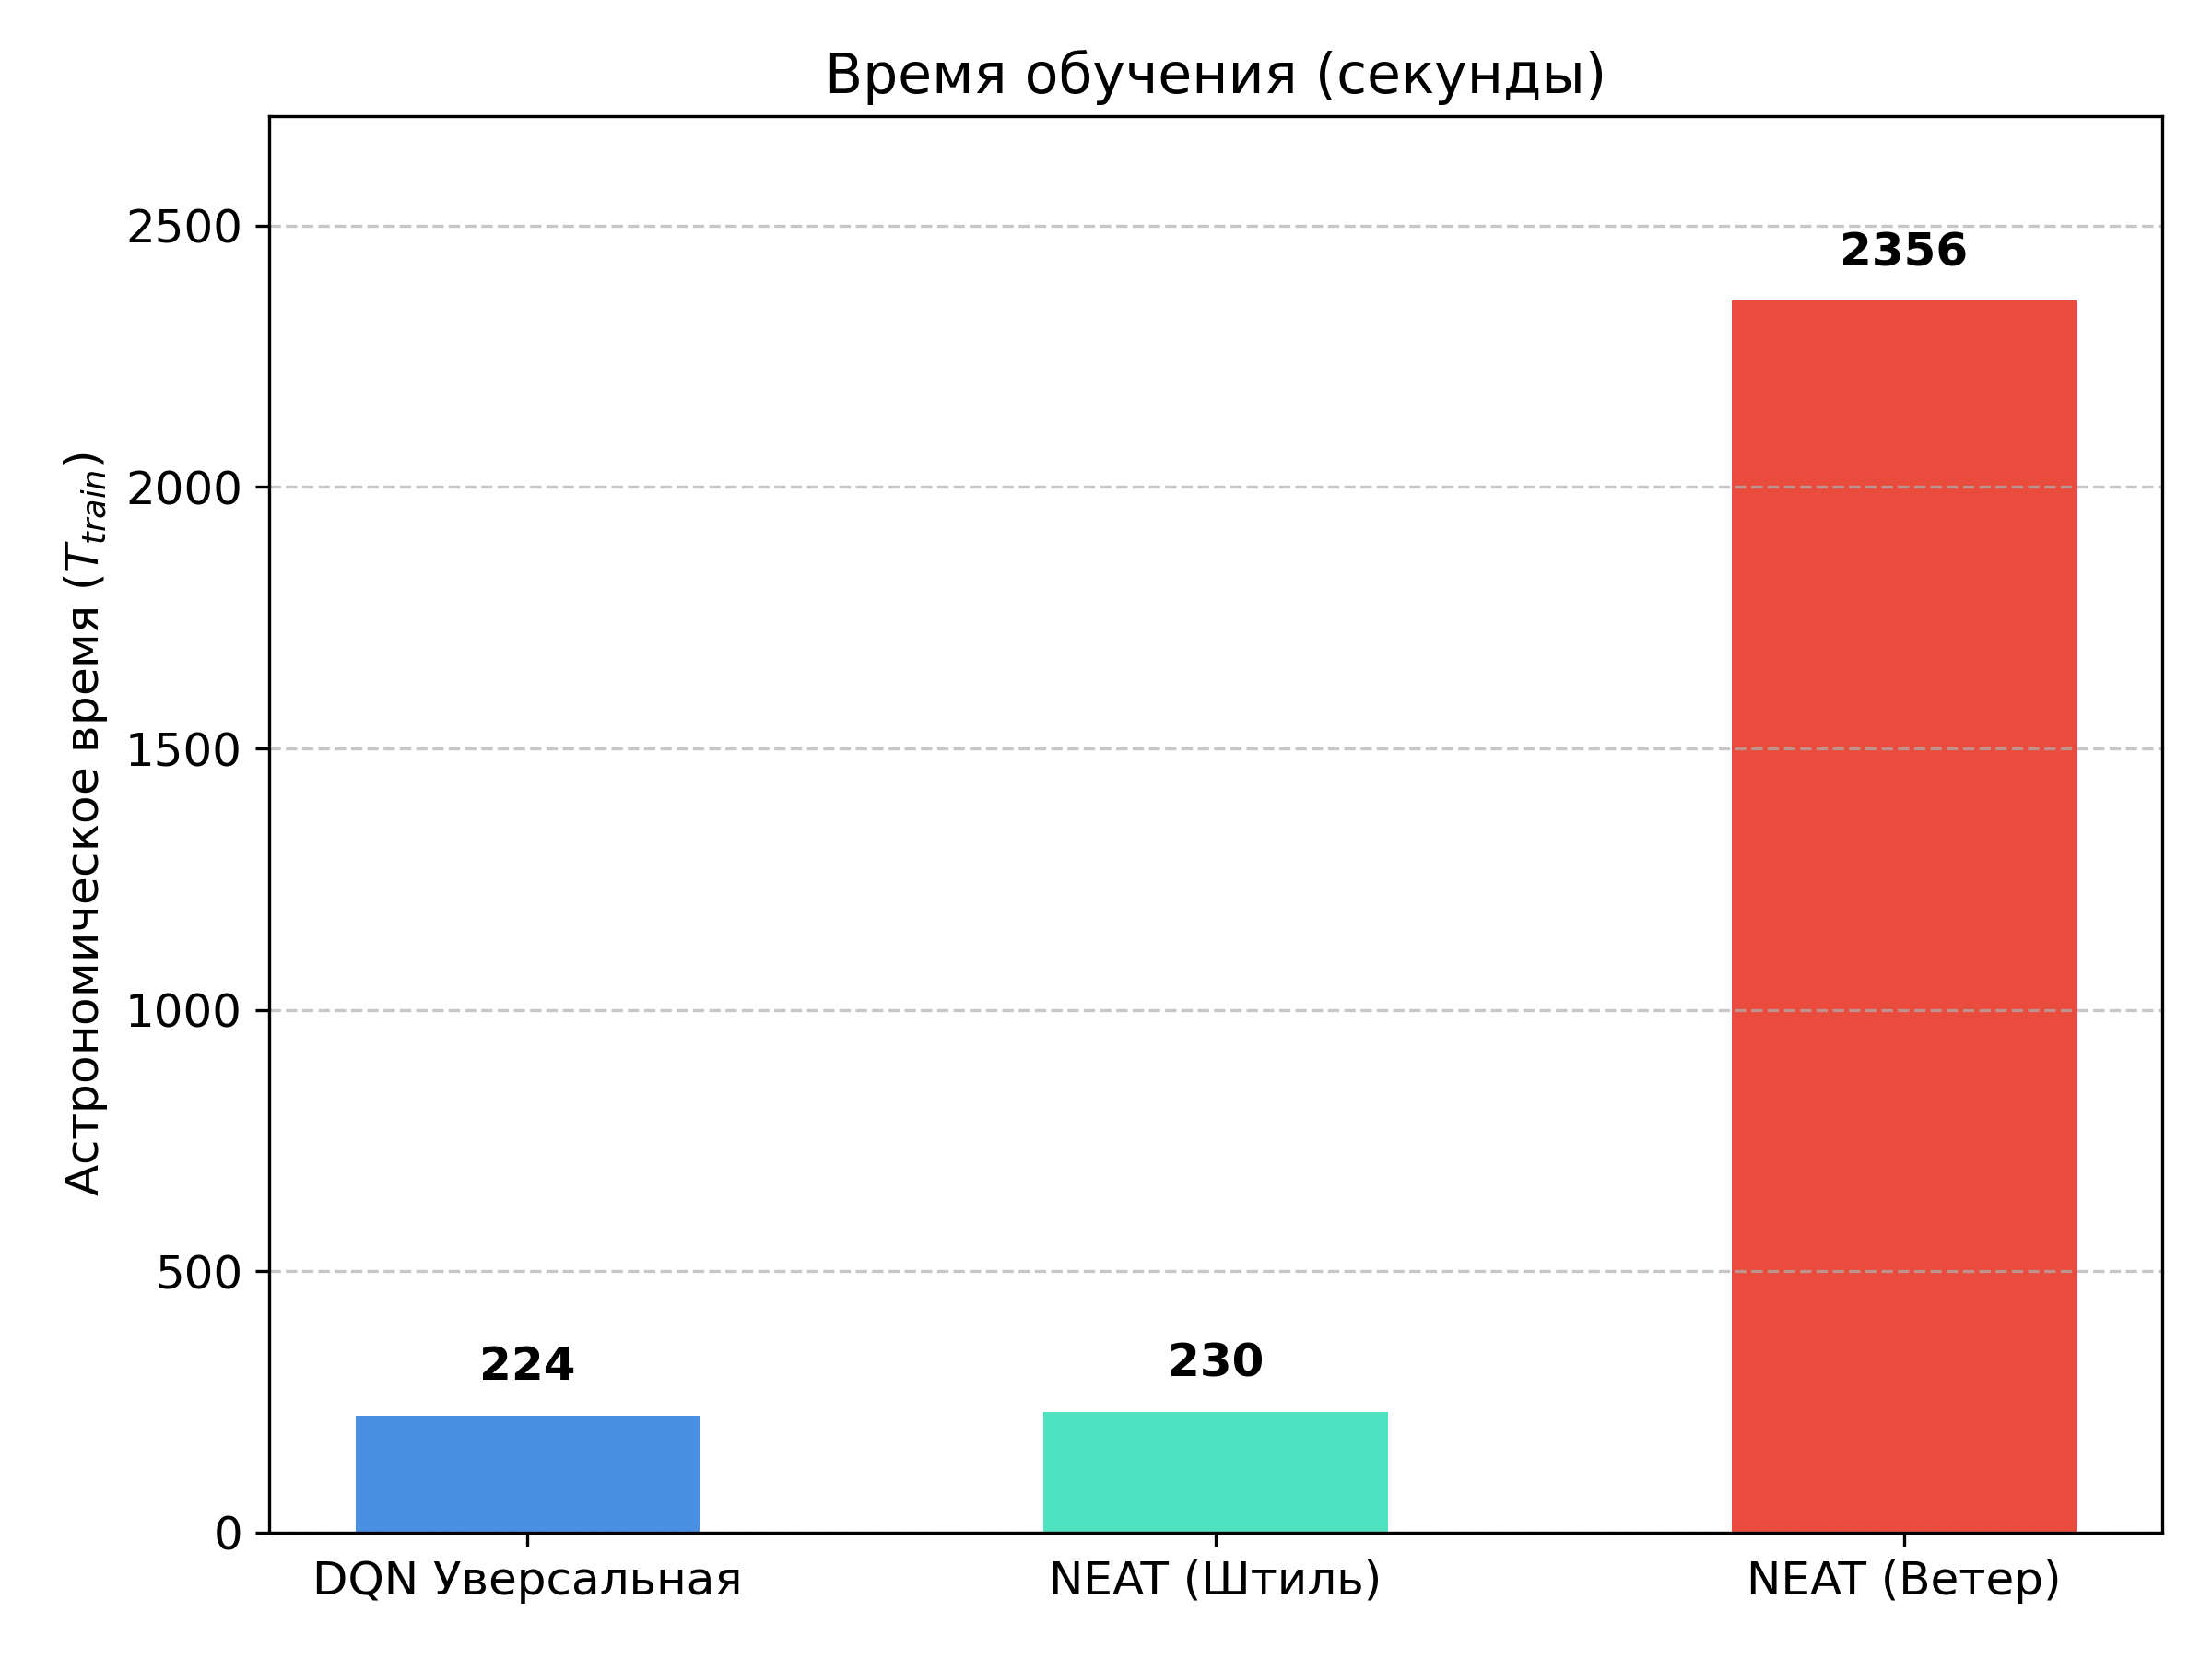
\includegraphics[width=0.6\textwidth]{./images/lunarlander_speed.png}
  
  \caption{Скорость схождения двух алгоритмов.}
  \label{fig:lunarlander_speed}
\end{figure}


Практика опять подтвердила гипотезу контрасте между тем, как алгоритмы формируют управляющую политику. Если смотреть на скорость схождения на рисунке \ref{fig:lunarlander_speed}, то алгоритм DQN оказался явным лидером, потому что пробил целевой порог приспособленности (>200) всего за 170 000 шагов взаимодействия со средой, что заняло около 224 секунд реального времени. Нейроэволюционному подходу потребовалось куда больше итераций для поиска рабочей топологии.  Однако эта задержка на этапе обучения полностью окупается в момент инференса. Итоговая информационная емкость моделей отличается на порядки, что можно увидеть на рисунке \ref{fig:lunarlander_complexity}. Для достижения стабильных результатов DQN-агенту понадобилась тяжеловесная глубокая сеть размерностью [512, 512], содержащая 69 124 обучаемых параметра. NEAT же, напротив, вырастил очень компактный граф всего из 150–200 связей и узлов.

\subsubsection{Феномен «нейролоботомии» и проблема локальных оптимумов}

Во время симуляций мы столкнулись с весьма специфическим побочным эффектом, который условно классифицировали как «нейролоботомию». Из-за того, что среда накладывает жесточайший штраф за крушение модуля в -100 очков, самый безопасный выход для развития адаптации агента к среде, но не менее деструктивный выход стал в том, чтобы вообще ничего не делать. Агент буквально обрывал связи в собственной сети и отключал двигатели, лишь бы не совершить фатальную ошибку при активном маневрировании. Статистически алгоритму было выгоднее просто падать вниз, чем пытаться управлять модулем и разбиваться. Чтобы вытащить сеть из этого локального оптимума, нам пришлось перенастраивать функции приспособленности и добавлять элементы рандомизации в стартовые условия.

\subsubsection{Устойчивость в условиях неопределенности и внешних шумов}

\begin{figure}[h!] % [h!] - попытка разместить картинку "здесь" (here)
  \centering
  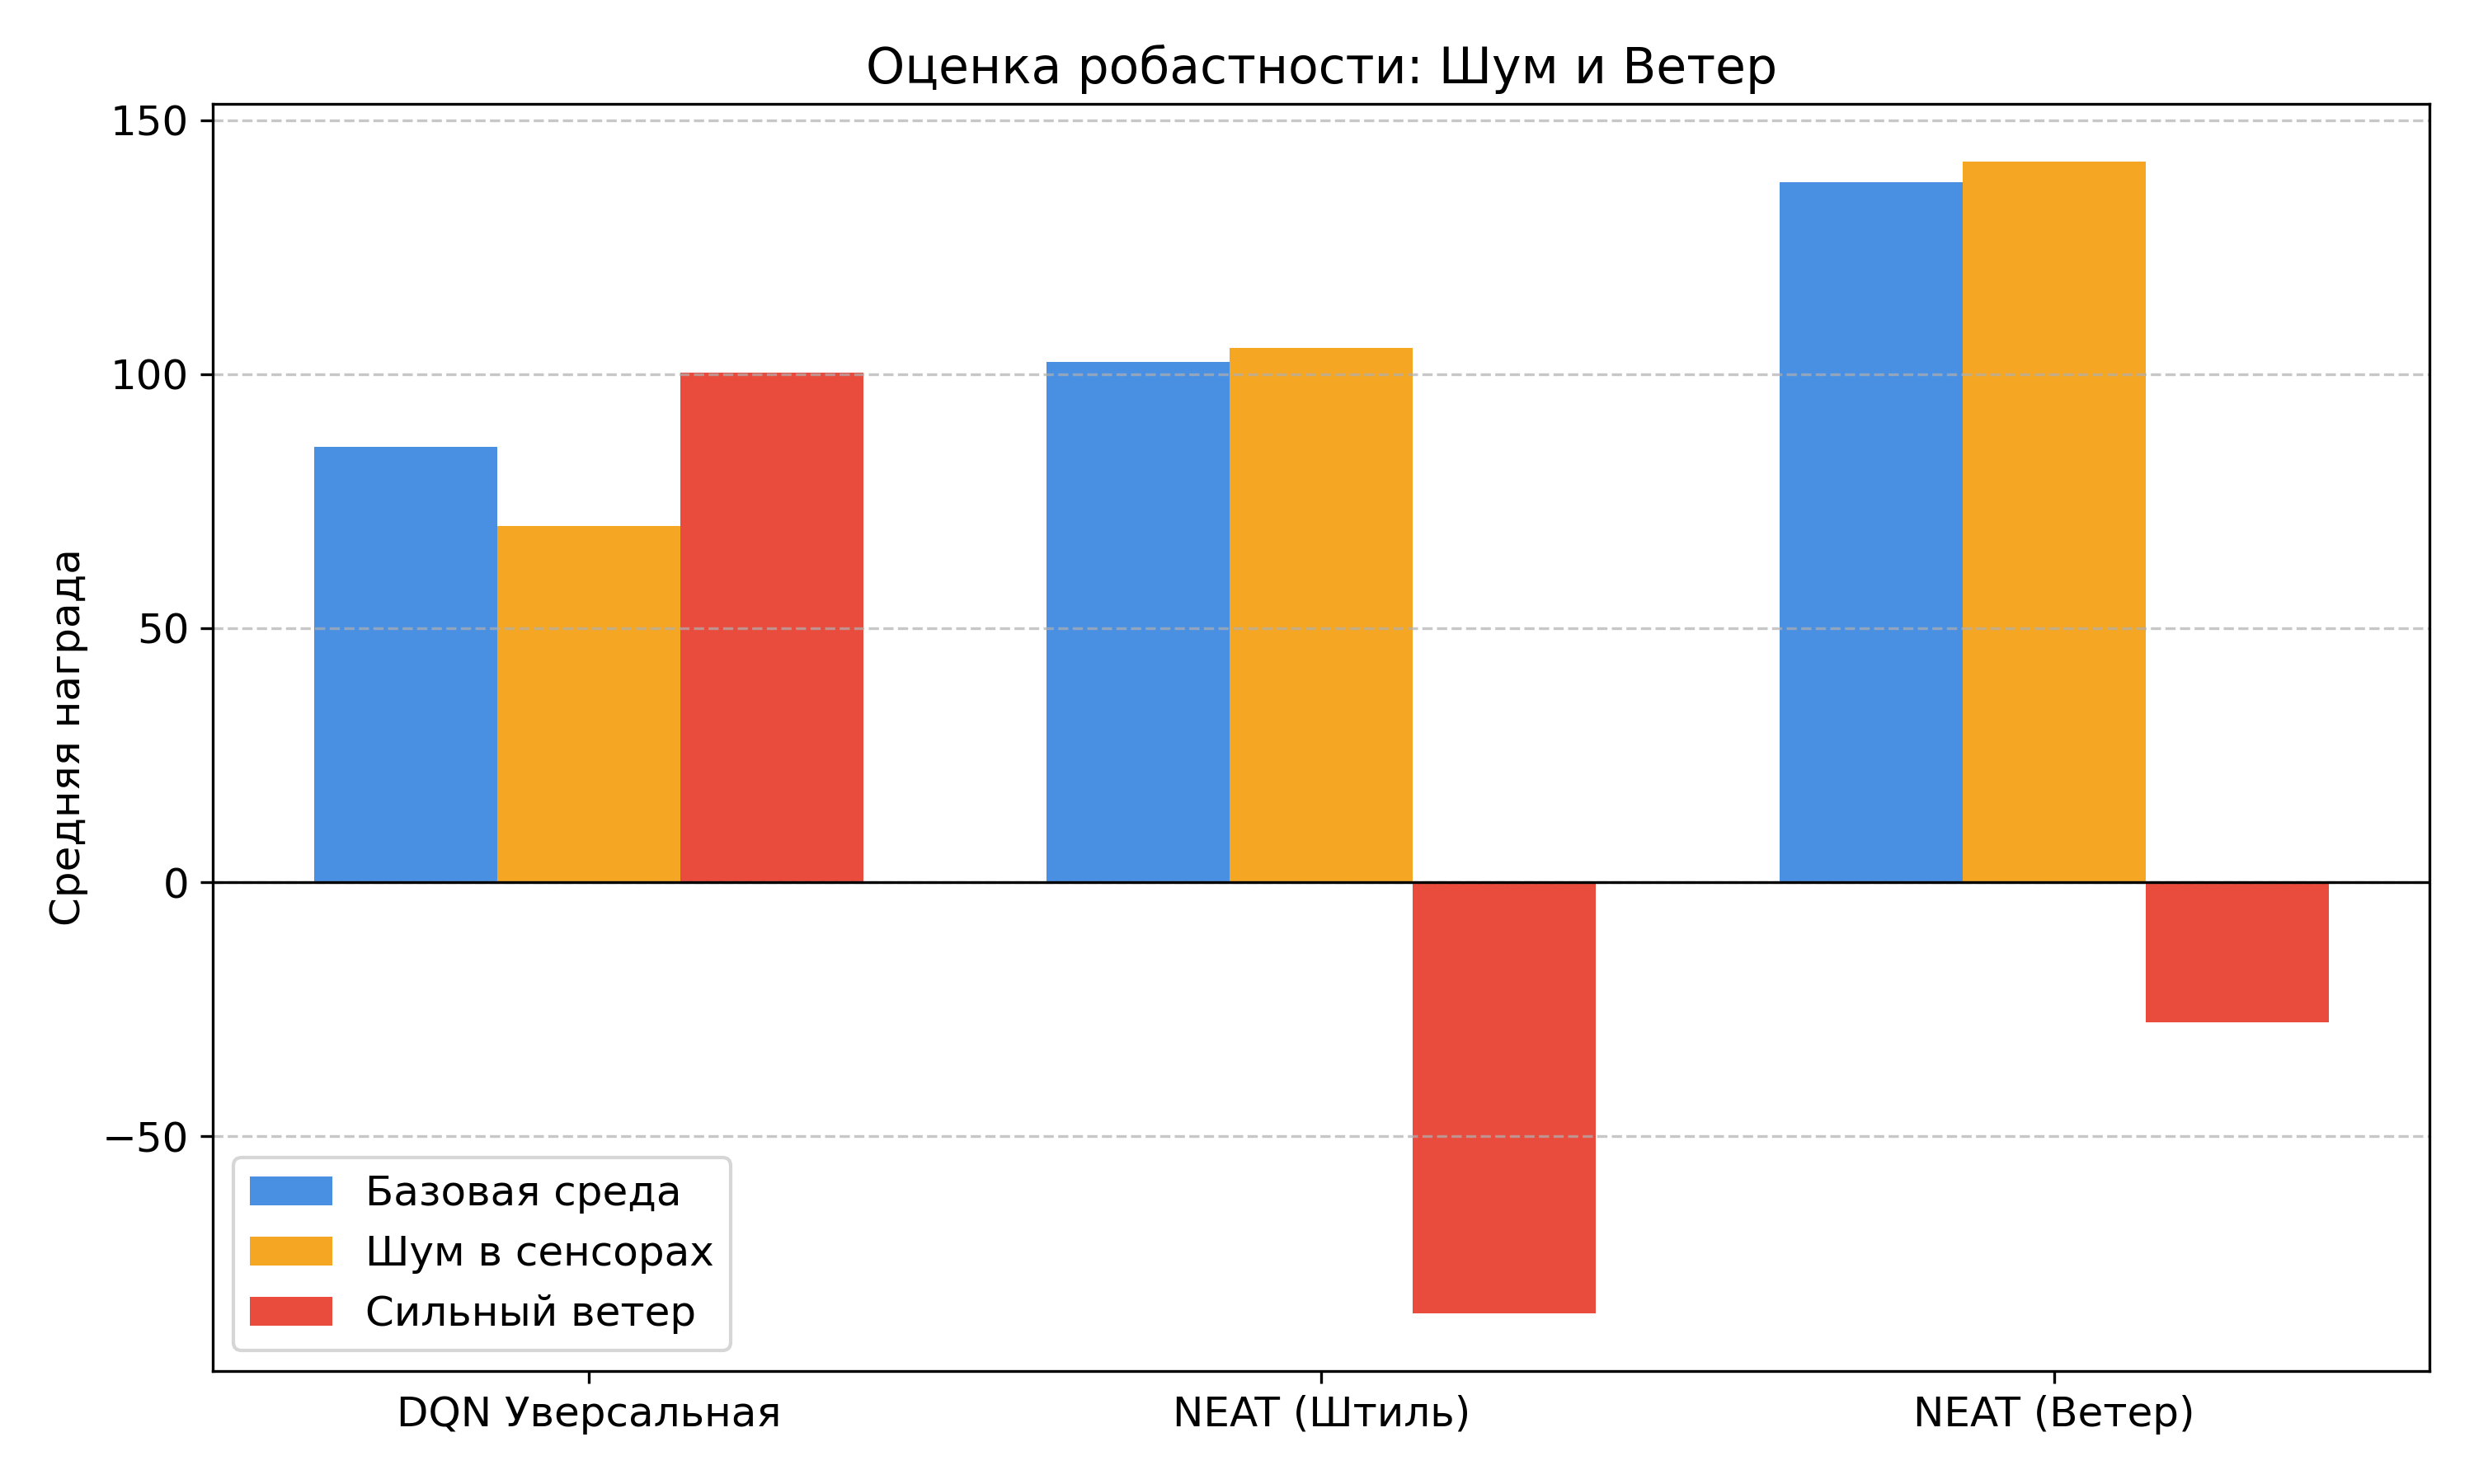
\includegraphics[width=0.6\textwidth]{./images/lunarlander_robustness.png}
  
  \caption{Устойчивость двух алгоритмов.}
  \label{fig:lunarlander_robustness}
\end{figure}

Отдельной задачей стало стресс-тестирование агентов на устойчивость к внешним возмущениям вроде турбулентности или бокового ветра. Для DQN пришлось написать специальную обертку UniversalWindWrapper, которая в половине эпизодов генерировала порывы ветра мощностью до 20.0. Это вынуждало полносвязную сеть искать паттерны компенсации смещения. С алгоритмом NEAT мы поступили иначе: заставили каждый геном сдавать серию из 5 испытаний (EPISODES\_PER\_GENOME = 5), где штиль чередовался с непогодой. Итоговая оценка суммировалась, а фактор случайного везения сводился к нулю. 

Сводные результаты этих тестов на рисунке \ref{fig:lunarlander_robustness} показывают, что универсальная DQN-модель отлично справляется в идеальных условиях, набирая 85.75, но слаба перед шумами в сенсорах, проседая по эффективности до 70.13. В то же время NEAT показал хорошую стабильность к высокочастотным помехам из-за низкой сложности архитектуры нейросети.

\subsubsection{Специфика программной реализации}

Чтобы гарантировать научную достоверность и воспроизводимость всех экспериментов, мы строго контролировали генерацию случайных чисел. Это ставило всю популяцию из 150-300 агентов в абсолютно идентичные стартовые условия, делая эволюционный отбор полностью равным. А учитывая тяжелую физику LunarLander и необходимость пятикратной проверки каждой особи, мы распараллелили вычисления по ядрам процессора через модуль multiprocessing.

\subsubsection{Практические выводы}

Классический подход DQN — это отличный выбор для быстрого обучения в детерминированной среде с высокой размерностью данных. Но если речь заходит о создании устойчивых систем управления, которым предстоит работать в условиях неопределенности и жесткого дефицита вычислительных ресурсов, нейроэволюция оказывается гораздо более предпочтительным инструментом.

\subsection{Результаты в среде Ant}

Экспериментальное исследование в среде симуляции четырехногого робота (Ant-v4) стало завершающим и наиболее технически сложным этапом практической части работы. Данная среда, базирующаяся на физическом движке MuJoCo, отличается высокоразмерным непрерывным пространством состояний и действий, что предъявляет экстремальные требования к архитектуре когнитивного агента.


\subsubsection{Обоснование выбора модальности обучения}

В отличие от сред CartPole и LunarLander, где проводился сравнительный анализ двух алгоритмов, моделирование в среде Ant-v4 осуществлялось исключительно с использованием нейроэволюционного подхода (NEAT). Данное ограничение было введено намеренно и обусловлено фундаментальными математическими ограничениями классического алгоритма глубокого Q-обучения (DQN).

Поскольку управление «муравьем» требует подачи непрерывных сигналов на 8 независимых суставов, применение DQN потребовало бы искусственной дискретизации пространства действий. Даже при минимальном разбиении (например, на 3 состояния: тянуть назад, покой, тянуть вперед) алгоритм столкнулся бы с проблемой комбинаторного взрыва — $3^8 = 6561$ уникальная комбинация действий на каждом такте. Нейроэволюционный алгоритм NEAT, напротив, способен напрямую генерировать векторы непрерывных управляющих сигналов, что делает его оптимальным выбором для задач робототехники в рамках данного исследования.


\subsubsection{Эволюция функции вознаграждения (Reward Shaping) и адаптация среды}

Процесс обучения агента в среде Ant-v4 потребовал глубокого инженерного вмешательства в механику симуляции. В ходе первичных запусков с базовыми настройками среды был зафиксирован феномен стагнации приспособленности (отрицательные значения от -30 до 0). Анализ логов показал, что агент попадал в локальный оптимум, который можно охарактеризовать как «отказ от действий».

Для достижения итогового результата — биомеханически корректного и эффективного движения — был применен метод последовательного усложнения функции вознаграждения (Reward Shaping):

\paragraph{Решение проблемы «штрафа за энергию» (ctrl\_cost):} В базовой версии среды любые резкие сигналы на суставы карались жестким штрафом, который превышал награду за выживание. Эволюция NEAT реагировала на это радикально — алгоритм намеренно «ломал» нейросеть (уменьшая её размерность), чтобы выдавать нулевые сигналы и не получать штрафы. Для преодоления этой проблемы весовые коэффициенты штрафов в коде инициализации среды были снижены, что позволило агенту начать первичные исследования моторики без риска мгновенного завершения эпизода.

\paragraph{Внедрение «умного таймера» стабилизации:} Муравей появлялся в воздухе и падал на поверхность. Базовый код убивал агента за отсутствие скорости (таймер лени) еще до того, как тот успевал сгруппироваться после падения. Была разработана система «умного таймера», предоставляющая агенту запас времени (150 тактов) на стабилизацию после приземления и поощряющая любое, даже самое незначительное, продвижение вперед (установка собственного рекорда дистанции).

\paragraph{Получение биомеханически правильной походки:} После того как агент научился не погибать на старте и хаотично перебирать конечностями (простая функция награды), система вознаграждения была переориентирована на максимизацию проекции скорости вектора центра масс по оси X при минимизации энергозатрат.




\subsubsection{Практические выводы}

Благодаря поэтапной модификации функции вознаграждения, алгоритм NEAT успешно синтезировал топологию нейронной сети, способную управлять сложной многозвенной системой.

Эволюционный процесс привел к отказу от хаотичных, судорожных движений в пользу скоординированной походки. Агент научился использовать инерцию собственного тела, синхронизируя работу 8 суставов для поддержания баланса и минимизации контакта корпуса с землей. Итоговая модель нейросети оказалась поразительно компактной (учитывая сложность задачи), продемонстрировав способность нейроэволюции находить элегантные решения в многомерных пространствах без избыточного наращивания вычислительных мощностей.